%<*figPipeline>
\begin{figure*}
	\centering
	\scalebox{0.9}{
		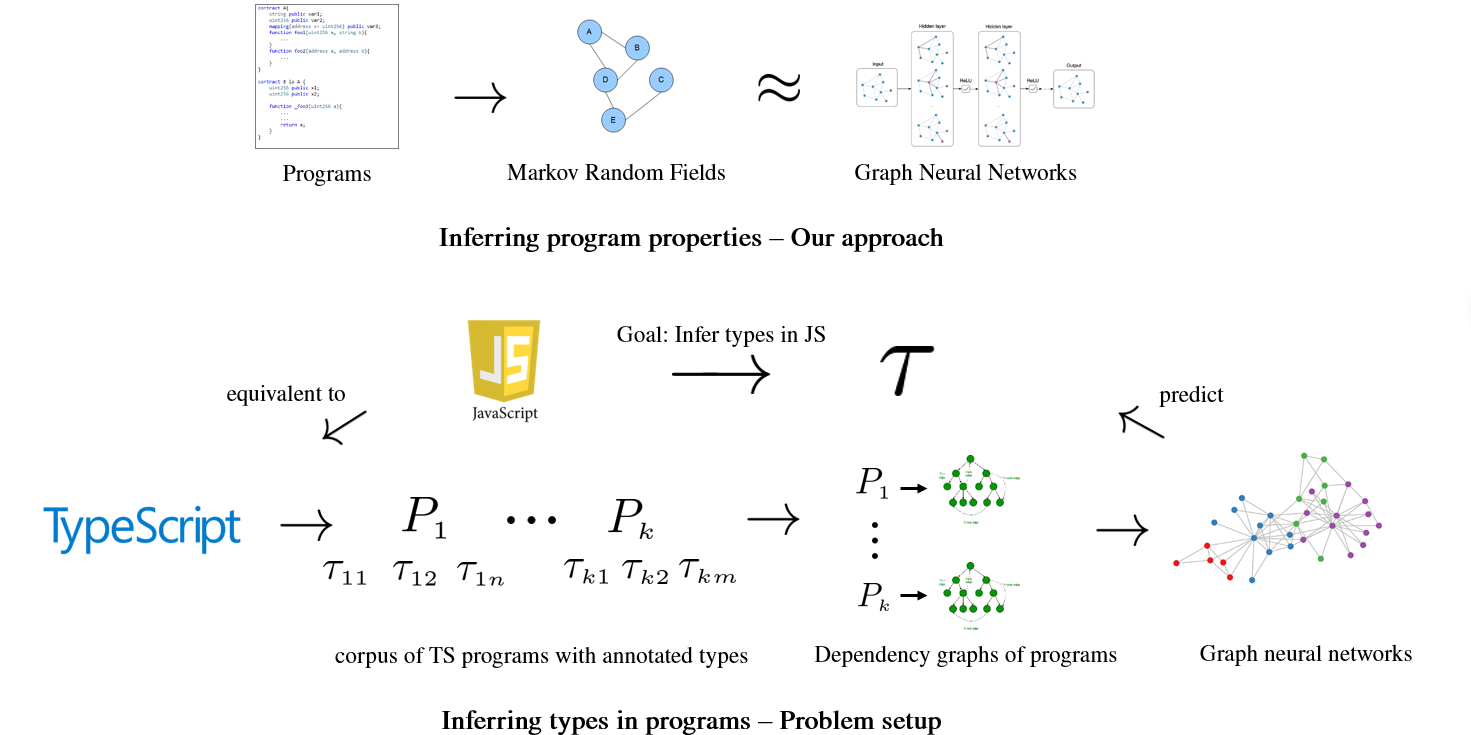
\includegraphics[width=\textwidth]{img/architecture.png}
	}
	\caption{\textbf{Summary of our work.} We motivate the problem of modeling programs as Markov Random Fields. We argue that a Graph neural network approximates inference tasks over an MRF. Specifically, we investigate the problem of inferring types in Javascript programs.}
	\label{fig:pipeline}
\end{figure*}
%</figPipeline>

%<*figSetup>
\begin{figure}
	\centering
	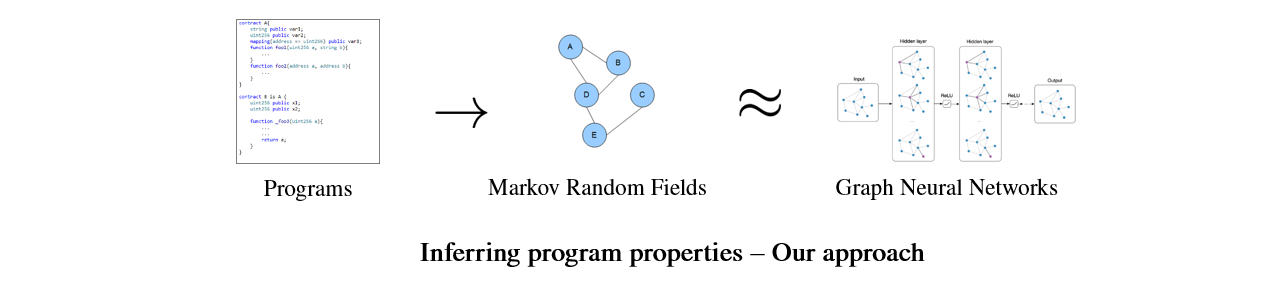
\includegraphics[width=\linewidth]{img/approach.png}
	\caption{Problem setup}
	\label{fig:setup}
\end{figure}
%</figSetup>

%<*gnn>
\begin{figure}
	\centering
	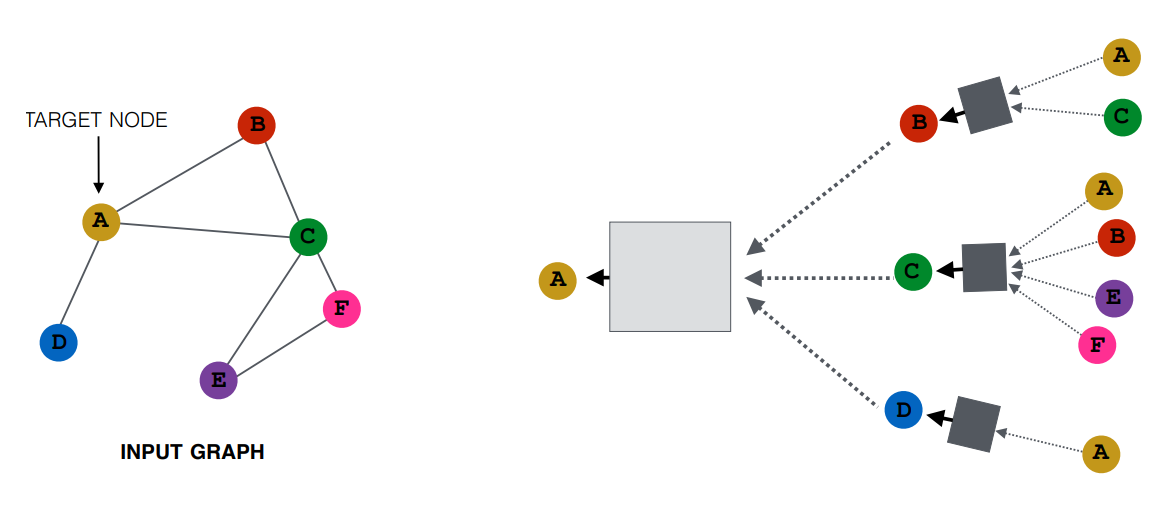
\includegraphics[width=\linewidth]{img/gnn.png}
	\caption{A typical graph neural network architecture. The key idea is to generate node embeddings based on neighborhood information. Image credit: Tutorial slides from \textit{Representation Learning on Networks}, held at WWW 2018.}
	\label{fig:gnn}
\end{figure}
%</gnn>

%<*stats>
\begin{figure}
	\centering
	\begin{subfigure}{0.15\textwidth}
		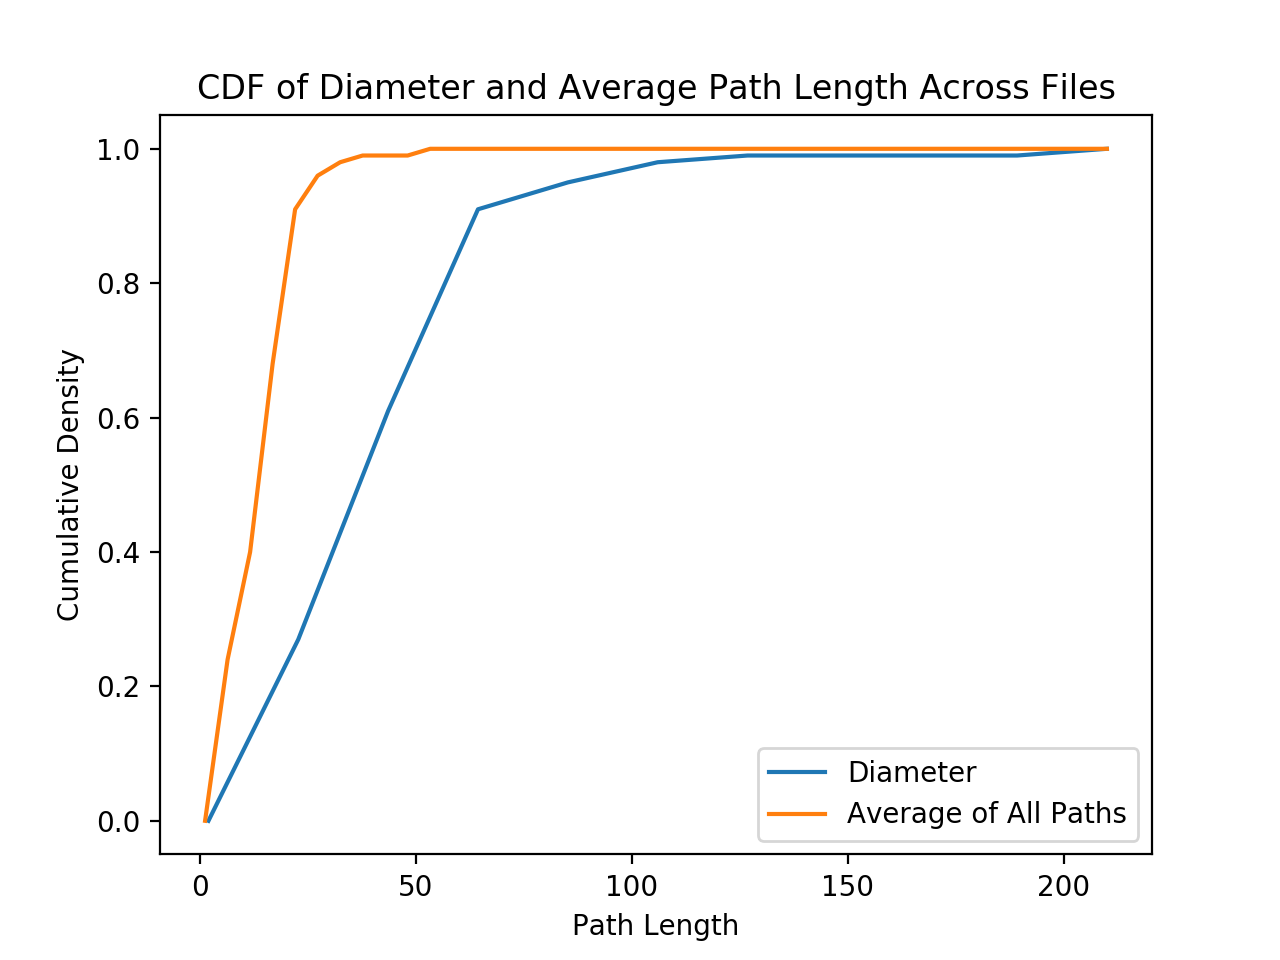
\includegraphics[width=\textwidth]{img/diameter}
		\label{fig:g1}
	\end{subfigure}
	\begin{subfigure}{0.15\textwidth}
		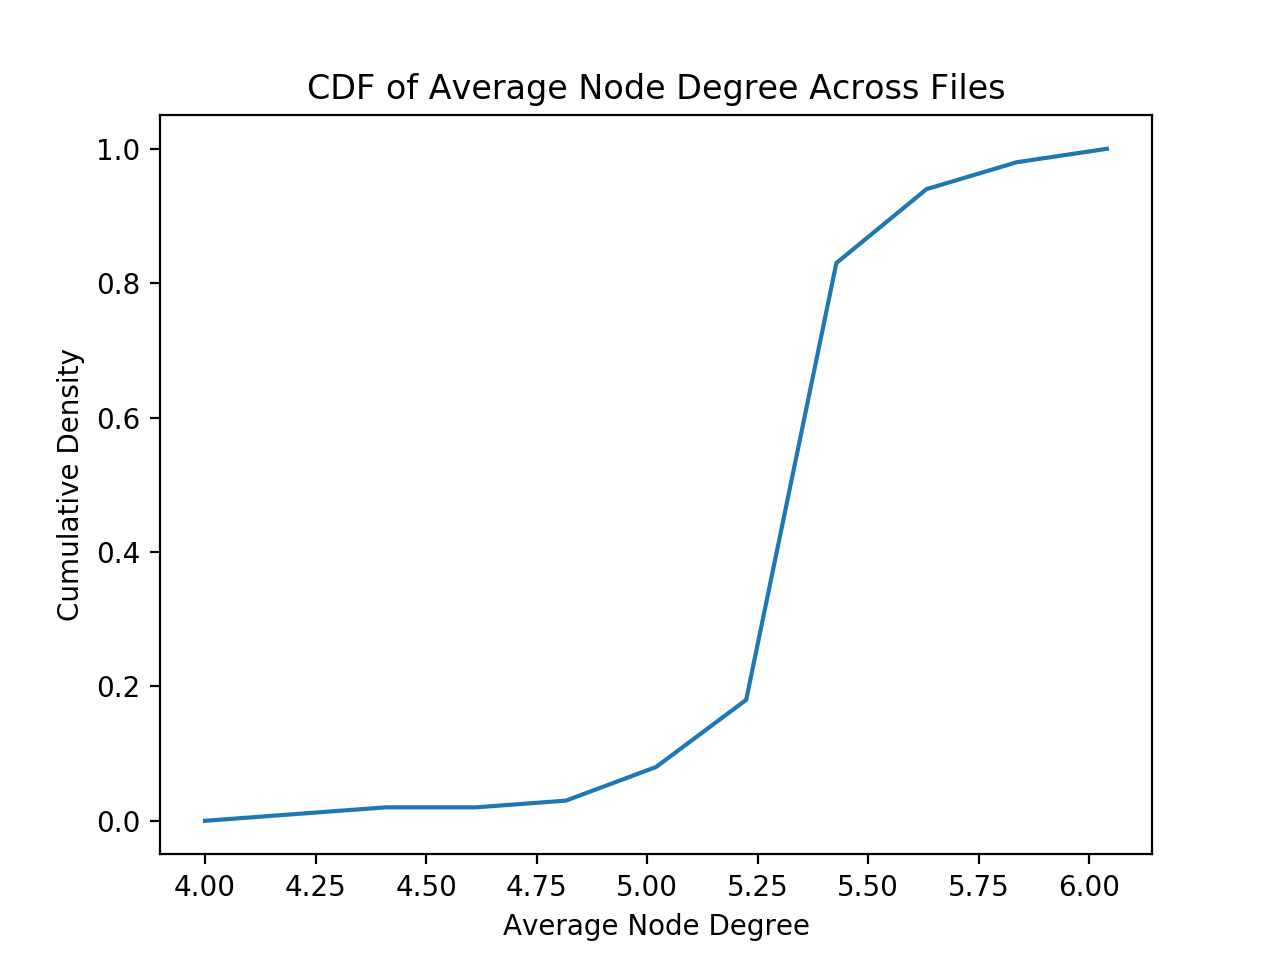
\includegraphics[width=\textwidth]{img/node_degree}
		\label{fig:g2}
	\end{subfigure}
	\begin{subfigure}{0.15\textwidth}
		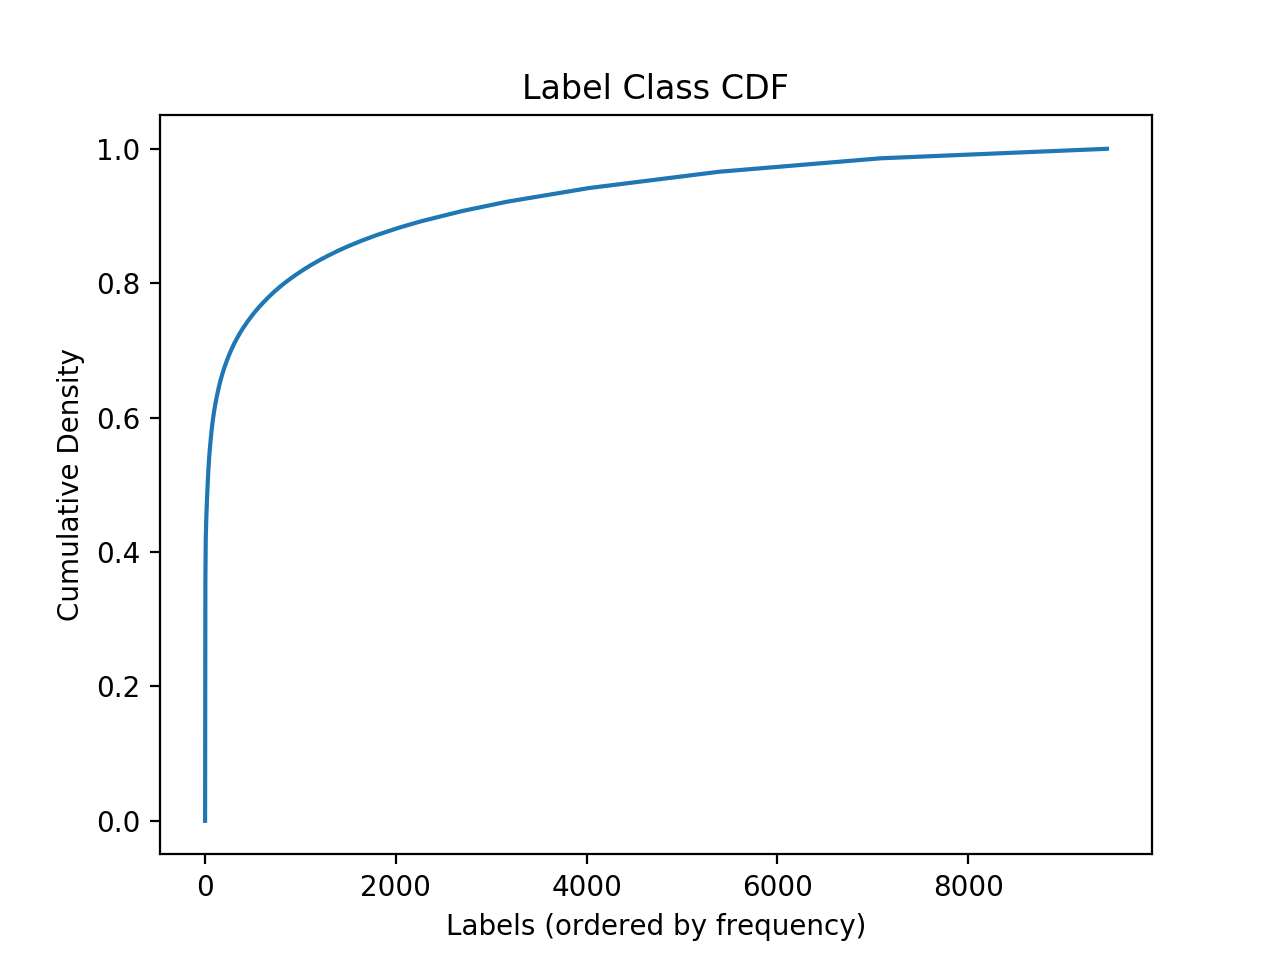
\includegraphics[width=\linewidth]{img/label_cdf}
	\end{subfigure}
	\caption{A summary of key dataset statistics. The first two plots show the CDFs of the average path length, and the node degrees of the graphs in the dataset. The third plot shows the CDF of the label distribution. }
	\label{fig:dataset-graph-stats}
\end{figure}
%</stats>

%<*gpDiagram>
\begin{figure}
	\centering
	\scalebox{0.7}{
	    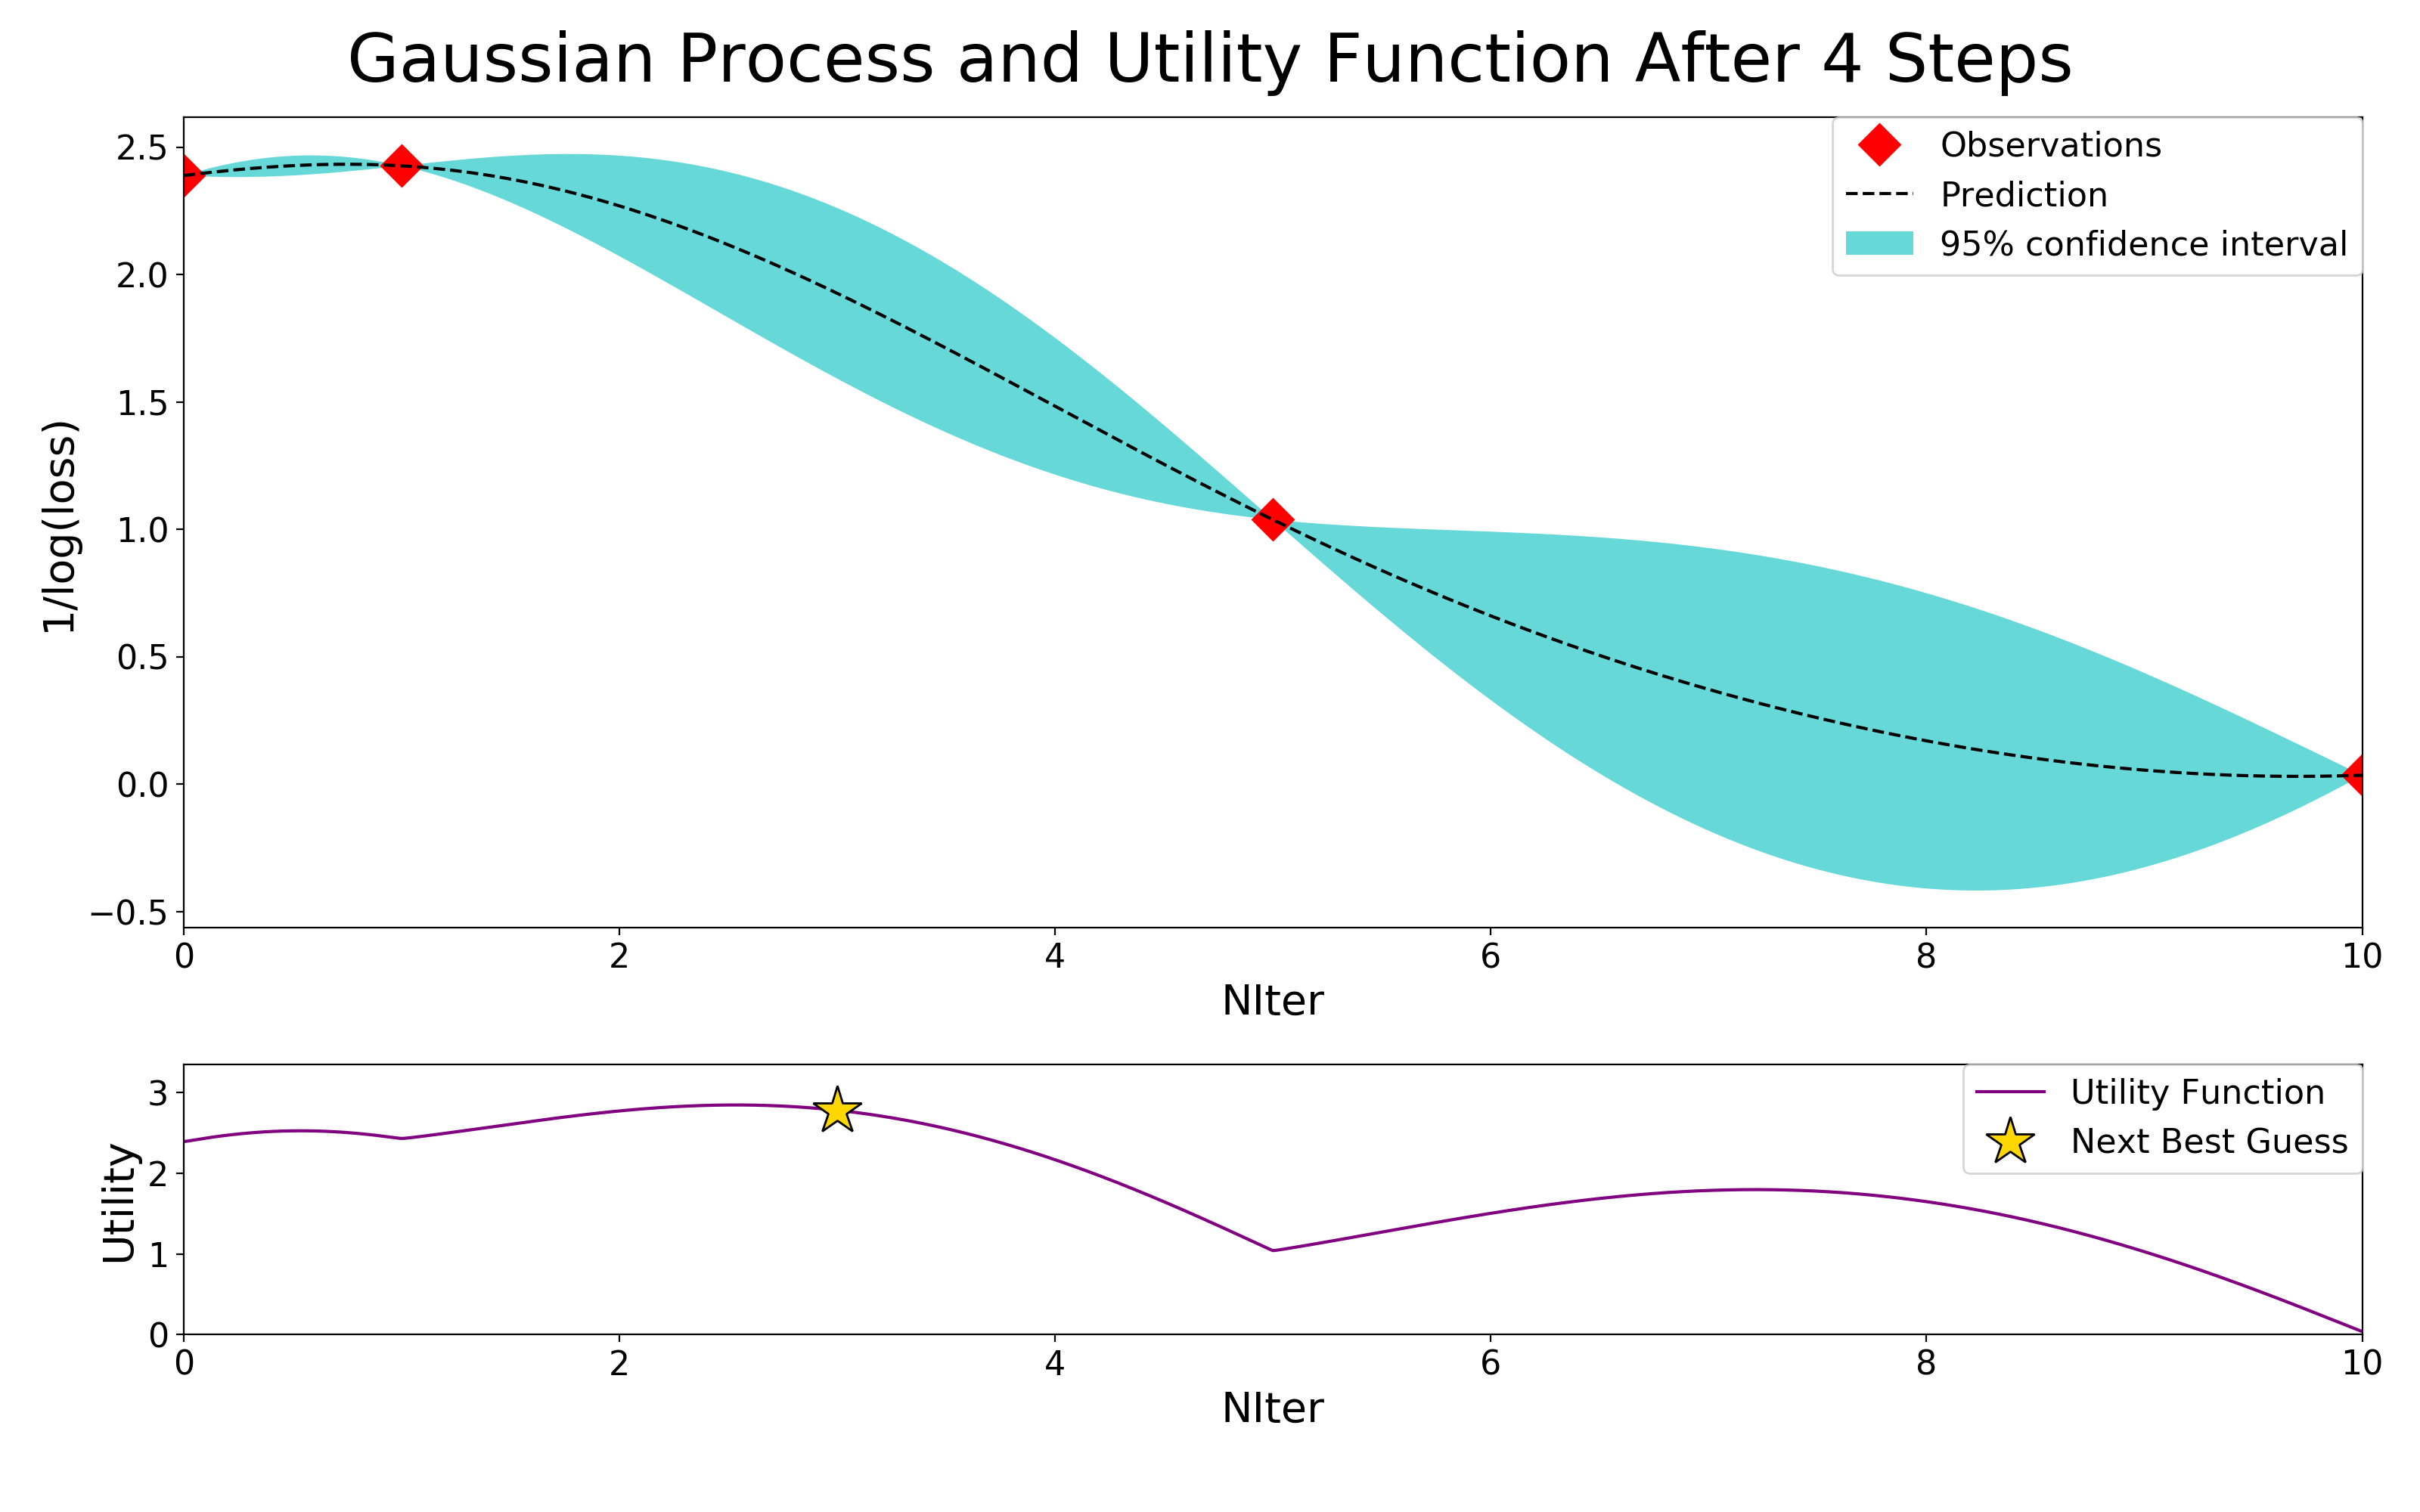
\includegraphics[width=\linewidth]{img/bo}
	}
	\caption{Partial result of Bayesian Optimization on \textsc{NIter} (after 4 samples)}
	\label{fig:gp-diagram}
\end{figure}
%</gpDiagram>

%<*graph>
\begin{figure}
	\centering
	\scalebox{0.7}{
		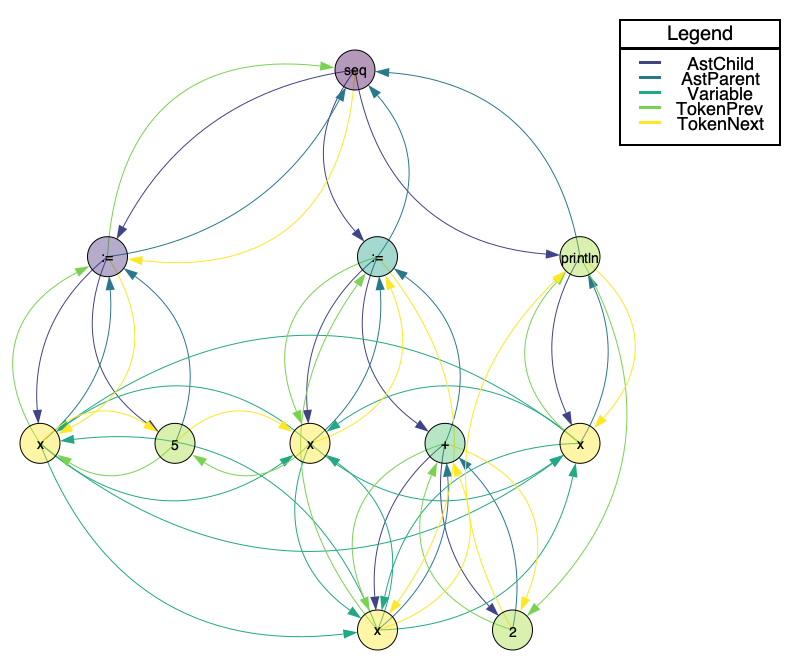
\includegraphics[width=\linewidth]{img/gen_graph}
	}
	\caption{Generated graph for a simple example}
	\label{fig:ast-graph}
\end{figure}
%</graph>

%<*mrf>
\begin{figure}
	\centering
	\scalebox{0.7}{
		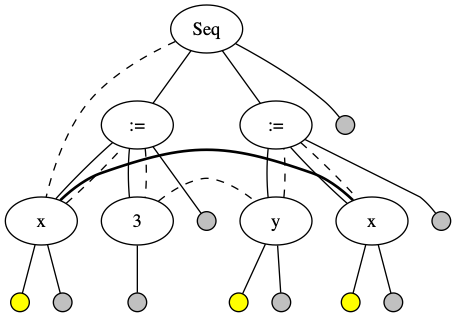
\includegraphics[width=\linewidth]{img/mrf_graph}
	}
	\caption{Markov Random Field for an example program. Shaded nodes are observed, highlighted are posteriors}
	\label{fig:mrf-graph}
\end{figure}
%</mrf>
